\documentclass[10pt,A4paper,tikz,border=10pt]{standalone}
\usepackage[utf8]{inputenc}
\usepackage[T1]{fontenc}
\usepackage{amsmath}
%\usepackage{amsfonts}
\usepackage{amssymb}
\usepackage{mathtools}
\DeclarePairedDelimiter\abs{\lvert}{\rvert}
\usepackage{tikz}
\usetikzlibrary{shapes,arrows,shapes.misc,shapes.symbols}
\usetikzlibrary{positioning}
\usepackage{gitinfo2}
\usepackage{graphicx}

\makeatletter
\AddToShipoutPictureBG{%
	\AtPageLowerLeft{%
		\kern2.6cm
		\raisebox{\dimexpr.5\paperheight-.8\height}
		{\rotatebox{90}{\gitMarkFormat\gitMarkPref{} \textbullet{} \gitMark}}%
	}%
}%
\makeatother
\newcommand{\prdfrazioni}{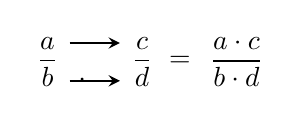
\begin{tikzpicture}[thick]
		\def\x{2.8mm}
		\def\h{2.4mm}
		\def\dist{12mm}%1cm
		\node at (0,0) {$\displaystyle \frac{a}{b}$};
		\node at (\dist,0) {$\displaystyle \frac{c}{d}$};
		\node at (1.4*\dist,0) {$\displaystyle =$};
		\node at (2.0*\dist,0) {$\displaystyle \frac{a\cdot c}{b\cdot d}$};
		% collegamento termini
		\draw[-stealth] (\x, \h)--(\dist-\x,\h); 
		\draw[-stealth] (\x,-\h)--node [near start] {$\cdot$}(\dist-\x, -\h);
	\end{tikzpicture}%
}
%\renewcommand{\gitMarkFormat}{\color{blue}\sffamily\bfseries}
\begin{document}
\tikzset{
	decision/.style={diamond, draw, %fill=blue!20,
		text width=5.5em, text badly centered, 
		%node distance=2.5cm
		, inner sep=0pt
	},
	block/.style={rectangle, draw, %fill=blue!20,
		text width=11.5em, 
		text centered, 
		%node distance=2.0cm,
		%rounded corners, 
		%minimum height=3em
	},
	loop/.style={chamfered rectangle,chamfered rectangle 	xsep=2cm, draw, %fill=blue!20,
		text width=15em, text centered,  
		node distance=2.5cm,% minimum height=3em
	},
	cloud/.style={draw, ellipse,%fill=red!20, 
		%node distance=1.5cm,
		 minimum height=2em
	},
	input/.style={ % requires library shapes.geometric
		draw,
		%node distance=1.5cm,
			text width=15em, text centered,  
		trapezium,
		trapezium left angle=60,
		trapezium right angle=120,
	},
	line/.style={draw, very thick, %color=black!50,
		-latex'},
	print/.style={ % requires library shapes.symbols
		draw,
		text width=14em, 
		text centered,  
		tape,
		tape bend top=none
	},
connessione/.style={
draw,
circle,
radius=5pt,
}
}


		\begin{tikzpicture}[scale=1, %node distance = 2.5cm,
			 auto]
		\node (zero) {Forma normale $ax^2+bx+c=0$};
			\node [cloud, below of=zero] (init) {Inizio};
			\node[connessione,below of=init] (nodo1) {};
			\node [decision, below of=nodo1,node distance=2cm] (decisione1) {L'equazione è in forma normale?};
			\node[block, right of=decisione1, node distance=4.5cm] (dec1No) {Sommo i termini simili};
			\node[block, below of=decisione1, node distance=3cm] (dec1Si) {Cerco il termine di secondo grado};
			\node [decision, below of=dec1Si,node distance=3cm] (decisione2) {
				Esiste un termine di secondo grado?};
			\node[block, right of=decisione2, node distance=4.5cm] (dec2No) {$a=0$ l'equazione non è di secondo grado};% goto stop
			\node[block, below of=decisione2, node distance=3cm] (dec2Si) {$a$ è la parte numerica del termine di secondo grado};
			\node[block, below of=dec2Si, node distance=2cm] (blocco1) {Cerco il termine di primo grado};
			\node [decision, below of=blocco1, node distance=3cm] (decisione3) {Esiste un termine di primo grado?};
\node[block, right of=decisione3, node distance=4.5cm,text width=1em,] (dec3No) {$b=0$};
%			\node [print, below of=decisione1,node distance=3cm] (sceltasi1) {La trascrivo uguale a sinistra (prima) dell'uguale};
%			\node [print, right of=decisione1,node distance=6cm] (sceltano1) {La trascrivo cambiata di segno a sinistra  (prima) dell'uguale};
%			\node[connessione,below of=sceltasi1,node distance=1.5cm] (nodo2) {};
%			\node [decision, below of=nodo2,node distance=2.0cm] (decisione2) {Arrivato a destra?};
%			\node[connessione,below of=decisione2,node distance=2cm] (nodo3) {};
%		\node [input, below of=nodo3,node distance=1cm] (passo3) {Leggo l'espressione da sinistra verso destra cercando i numeri};
%		\node [decision, below of=passo3,node distance=2.8cm] (decisione3) {Il numero è a sinistra (prima) dell'uguale?};
%	\node [print, below of=decisione3,node distance=3cm] (sceltasi3) {La trascrivo cambiato di segno a destra (dopo) dell'uguale};
%\node [print, right of=decisione3,node distance=5.5cm] (sceltano3) {La trascrivo uguale a destra  (dopo) dell'uguale};
%\node[connessione,below of=sceltasi3,node distance=1.5cm] (nodo4) {};
%\node [decision, below of=nodo4,node distance=2cm] (decisione4) {Arrivato a destra?};
%\node[block,below of=decisione4,node distance=2.5cm] (passo4) {Sommo le incognite, Sommo i numeri};
%\node[decision,below of=passo4,node distance=3cm] (decisione5) {La somma delle incognite è zero?};
%\node[decision,right of=decisione5,node distance=4cm] (decisione6) {La somma dei numeri è zero?};
%\node[print,right of=decisione6, node distance =5cm] (sceltasi6) {Equazione indeterminata};
%\node[print,below of=decisione6, node distance =2.5cm] (sceltano6) {Equazione impossibile};
%\node[print,left of=decisione5, node distance =5.0cm] (sceltano5) {Equazione determinata};
%\node[print,below of=sceltano5, node distance =2cm] (passo5) {Soluzione $x=\displaystyle \frac{b}{a}$};
%\node[connessione,below of=sceltano6] (nodo5) {};
%	\node [cloud, below of=nodo5] (stop) {Fine};
%			\path [line] (init) -- (passo1);
%			\path [line] (passo1) -- (nodo1);
%     		\path [line] (nodo1) --  (passo2);
%    		\path [line] (passo2) --  (decisione1);
%     		\path [line] (decisione1) -- node[near start] {No} (sceltano1);
%     		\path [line] (decisione1) -- node[near start] {Si} (sceltasi1);
%			\path [line] (sceltasi1) --  (nodo2);
%			\path [line] (sceltano1) |-  (nodo2);
%			\path[line]  (nodo2)--(decisione2);
%			\path[line] (decisione2.west)--node[near start]{No}++(-3,0)|-(nodo1);
%			\path [line] (decisione2) --node[near start]{Si}  (nodo3);
%			\path [line] (nodo3) --  (passo3);
%			\path[line] (passo3)--(decisione3);
%			\path [line] (decisione3) -- node[near start] {No} (sceltano3);
%			\path [line] (decisione3) -- node[near start] {Si} (sceltasi3);
%			\path[line] (sceltasi3)--(nodo4);
%			\path[line] (sceltano3)|-(nodo4);
%			\path[line] (nodo4)--(decisione4);
%			\path[line] (decisione4.west)--node[near start]{No}++(-3,0)|-(nodo3);
%			\path[line] (decisione4)--(passo4);
%			
%				\path[line] (passo4)--(decisione5);
%				\path[line] (decisione5)--node [near start]{Si}(decisione6);
%				\path[line] (decisione6)--node [near start]{Si}(sceltasi6);
%				\path[line] (decisione6)--node [near start]{No}(sceltano6);
%			\path[line] (decisione5)--node [near start]{No}(sceltano5);
%			\path[line] (sceltano5)--(passo5);
%			\path[line](passo5)|-(nodo5);
%			\path[line] (sceltano6)--(nodo5);
%			\path[line] (sceltasi6)|-(nodo5);
%			\path[line](nodo5)--(stop);
		\end{tikzpicture}
\end{document}